\documentclass[a4paper,10pt]{scrartcl}

\usepackage{polski}
\usepackage[utf8]{inputenc}
\usepackage{graphicx}
\usepackage{enumerate}
\usepackage{pdflscape}

\title{Laboratorium 8}
\author{Filip Malinowski}
\date{\today}

\pdfinfo{%
  /Title    (Laboratorium 8)
  /Author   (Filip Malinowski)
}

\begin{document}

\title{Sprawozdanie z laboratorium 8}
\author{Filip Malinowski}
\date{\today}

\maketitle

Do programu zostały dodane drzewo binarne oraz
drzewo czerwono-czarne.
Drzewo czerwono-czarne niestety nie jest poprawnie
napisane. Przy próbie dodania elementów pojawia się
segmentation fault. Nie zdołałem poprawić tego błędu.

Złożoność obliczeniowa dodawania elementów do
binarnego drzewa poszukiwań powinna wynosić
\begin{math}
  n^{3}.
\end{math}
Zgadza się to z pomiarami.

Złożoność obliczeniowa odczytu w binarnym
drzewie poszukiwań powinna wynosić
\begin{math}
 n*log(n).
\end{math}
Również zgadza się to z pomiarami.

\pagebreak

\begin{landscape}
\begin{figure}
 \centering
 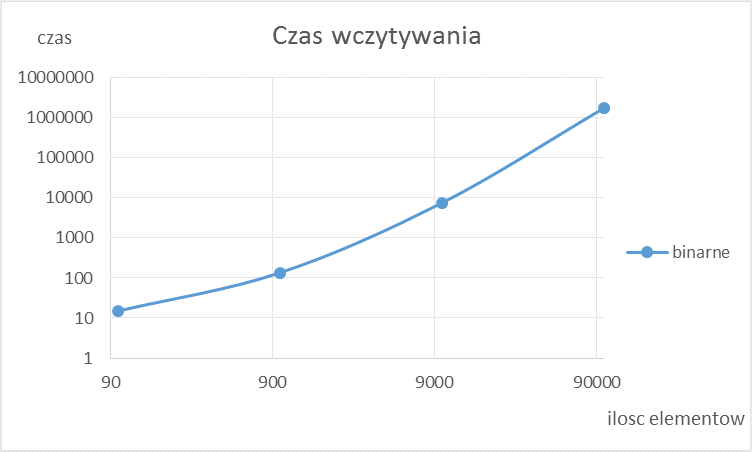
\includegraphics{wczytywanie}
 \caption{Wykres złożoności obliczeniowej wczytywania}
\end{figure}

\begin{figure}
 \centering
 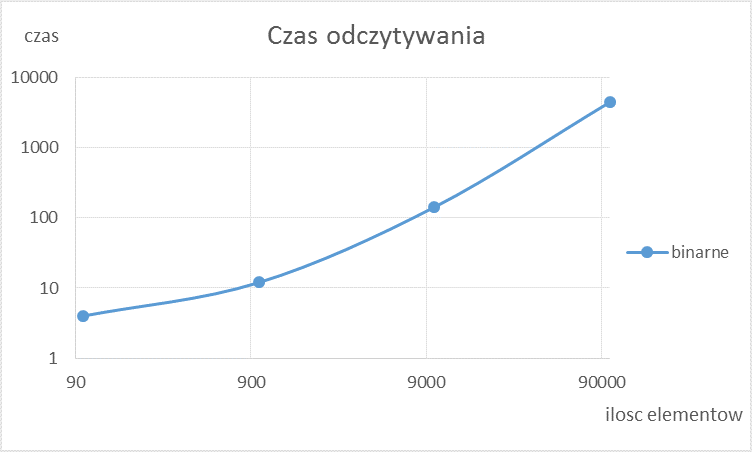
\includegraphics{odczytywanie}
 \caption{Wykres złożoności obliczeniowej odczytywania}
\end{figure}

\end{landscape}


\end{document}